%----------------------------------------------------------------------------------------
%	SOLUTION 5
%----------------------------------------------------------------------------------------
\newpage
\subsection*{Problem 5}
%----------------------------------------------------------------------------------------
%	SOLUTION 5.a
%----------------------------------------------------------------------------------------
\paragraph{5.a} Fig.~\ref{fig:q5_population_cov} shows the  Forward and smoothed a posteriori covariance of population error estimation for 10 time steps.
%%%%%%%%%%%%%%%%%%%%%%% POPULATION COV GRAPH %%%%%%%%%%%%%%%%%%%%%
\begin{figure}[!h]
	\centering
	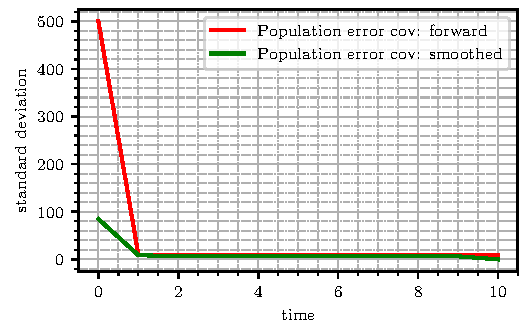
\includegraphics[scale=1.0,trim={0cm 0cm 0cm 0cm},clip]{./code/generatedPlots/q5_population_cov.pdf}
	\caption{Q5.a: Forward and smoothed a posteriori covariance of population error estimation for 10 time steps}
	\label{fig:q5_population_cov}
\end{figure}
Fig.~\ref{fig:q5_food_cov} shows the  Forward and smoothed a posteriori covariance of food supply error estimation for 10 time steps.
%%%%%%%%%%%%%%%%%%%%%%% FOOD COV GRAPH %%%%%%%%%%%%%%%%%%%%%
\begin{figure}[!h]
	\centering
	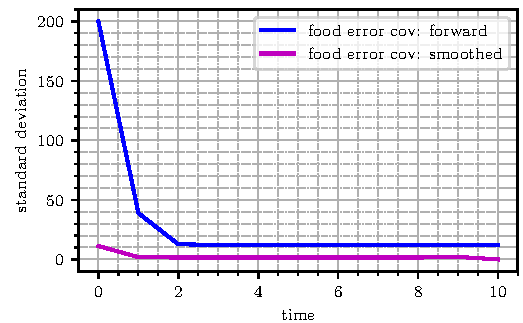
\includegraphics[scale=1.0,trim={0cm 0cm 0cm 0cm},clip]{./code/generatedPlots/q5_food_cov.pdf}
	\caption{Q5.a: Forward and smoothed a posteriori covariance of population error estimation for 10 time steps}
	\label{fig:q5_food_cov}
\end{figure}
%----------------------------------------------------------------------------------------
%	SOLUTION 5.b
%----------------------------------------------------------------------------------------
\paragraph{5.b}
Percentage improvement in the population estimation error variance due to smoothing at initial time is $490.09$\%.

Percentage improvement in the food supply estimation error variance due to smoothing at initial time is $1687.64$\%.

Improvement in food supply estimation at initial time is more because we do not measure food supply as we do for population, in which case measurement noise plays a role. Measurement noise degrades the estimate of the smoother in case of population. This is the reason of higher improvement percentage of food supply error estimation covariance at the initial time.
%----------------------------------------------------------------------------------------
%	SOLUTION 5.c
%----------------------------------------------------------------------------------------
\paragraph{5.c}Table~\ref{tbl:q5_init_cov} shows the numerical and theoretical state estimation error covariance for both the states.
%%%%%%%%%%%%%%%%%%%%%%%%%% TRAIN+VAL LINEAR MEAN ERROR %%%%%%%%%%%%%%%%%%%%%%%%%%%%%%%%%%%
\begin{table}[ht]
	\centering
	\caption{Q5: Numerical and theoretical initial state estimatiom error covariance}
	\begin{tabular}[t]{ccc} 
		\hline
		State 			& Numerical & Theoretical from part(b)\\ [0.5ex] 
		\hline
		Population 	& $84.73$ 	& $84.73$\\
		Food 	& $11.18$ 	& $11.18$\\[1ex]
		\hline
	\end{tabular}
	\label{tbl:q5_init_cov}
\end{table}
Thus from Table~\ref{tbl:q5_init_cov} we can see that both the numerical and theoretical estimates are close to each other, therefore, we can see one of the advantages of using smoother.
 